% !TeX program = xelatex

\documentclass[12pt, letterpaper]{report}
\usepackage[hmargin=1in, vmargin=1in]{geometry}
\usepackage{hyphenat}
\usepackage{ragged2e}

\newlength\tindent
\setlength{\tindent}{\parindent}
\setlength{\parindent}{0pt}
\renewcommand{\indent}{\hspace*{\tindent}}

\usepackage{fontspec}
\setmainfont[Ligatures=TeX]{Cambria}

\usepackage{amsfonts}
\usepackage{amssymb}
\usepackage{amsmath}

\usepackage{nccmath}

\usepackage{graphicx}
\usepackage{grffile}

\begin{document}

\setlength{\abovedisplayskip}{0pt}
\setlength{\belowdisplayskip}{0pt}
\setlength{\abovedisplayshortskip}{0pt}
\setlength{\belowdisplayshortskip}{0pt}

\makebox[\linewidth]{\rule{\textwidth}{0.4pt}}\\
\\\textbf{Problem A}\\
Find the roots of $f(x) = (e^x - e^\pi)(e^x - \pi)$ where $e$ denotes Euler's number.\\

Answer:\\
We denote the set of real numbers and integers by $\mathbb{R}$ and $\mathbb{Z}$ respectively.\\
Since it is not mentioned, we assume that we are not only finding $x\in\mathbb{R}$ but all $x\ni f(x) = 0$.\\

The roots of $f(x)$ are $x$'s such that $f(x) = 0 \Leftrightarrow (e^x - e^\pi)(e^x - \pi) = 0$.\\
This implies that either $e^x - e^\pi = 0$ or $e^x - \pi = 0$.\\

Let $x = p + iq$ where $p,q\in\mathbb{R}$ and $i$ is the imaginary unit.\\

If $e^x - e^\pi = 0$, then we have:

\begin{equation*}
e^x = e^\pi \Leftrightarrow e^{p+iq} = e^\pi \Leftrightarrow e^p e^{iq} = e^\pi
\end{equation*}

Since $q\in\mathbb{R}$, then by Euler's formula, $e^{iq} = \cos{q} + i\sin{q}$, hence:

\begin{equation*}
e^p e^{iq} = e^\pi \Leftrightarrow e^p(\cos{q} + i\sin{q}) = e^\pi \Leftrightarrow e^p \cos{q} + ie^p \sin{q} = e^\pi
\end{equation*}

This implies that $e^p \cos{q} = e^\pi$ and $ie^p \sin{q} = 0$ simultaneously.

Since $e^p\neq 0$ for an arbitrary $p\in\mathbb{R}$, then we find that $\sin{q}=0\Leftrightarrow q = 2n\pi, n\in\mathbb{Z}$.

This means that $\cos{q} = \cos{2n\pi} = 1$. So, $e^p\cos{q} = e^\pi\Leftrightarrow e^{p} = e^\pi\Leftrightarrow p = \pi$.

Hence, for $e^x - e^\pi = 0$, we have $x = p + iq = \pi + i\cdot 2n\pi = \pi + 2in\pi, n\in\mathbb{Z}$.\\

If $e^x - \pi = 0$, then we have:

\begin{equation*}
e^x = \pi \Leftrightarrow e^{p+iq} = \pi \Leftrightarrow e^p e^{iq} = \pi
\end{equation*}

Since $q\in\mathbb{R}$, then by Euler's formula, $e^{iq} = \cos{q} + i\sin{q}$, hence:

\begin{equation*}
e^p e^{iq} = \pi \Leftrightarrow e^p(\cos{q} + i\sin{q}) = \pi \Leftrightarrow e^p \cos{q} + ie^p \sin{q} = \pi
\end{equation*}

This implies that $e^p \cos{q} = \pi$ and $ie^p \sin{q} = 0$ simultaneously.

Since $e^p\neq 0$ for an arbitrary $p\in\mathbb{R}$, then we find that $\sin{q}=0\Leftrightarrow q = 2k\pi, k\in\mathbb{Z}$.

This means that $\cos{q} = \cos{2k\pi} = 1$. So, $e^p\cos{q} = \pi\Leftrightarrow e^{p} = \pi\Leftrightarrow p = \ln{\pi}$.

Hence, for $e^x - \pi = 0$, we have $x = p + iq = \ln{\pi} + i\cdot 2k\pi = \ln{\pi} + 2ik\pi, k\in\mathbb{Z}$.\\

This means the roots of $f(x) = (e^x - e^\pi)(e^x - \pi)$ are the sets:

{\centering
	$\{\pi + 2in\pi: n\in\mathbb{Z}\}${ } and { }$\{\ln{\pi} + 2ik\pi: k\in\mathbb{Z}\}$
\par}

\bigskip

$\therefore$ The roots of $f(x) = (e^x - e^\pi)(e^x - \pi)$ are given by the set:

\begin{equation*}
\{x: f(x) = 0\} = \{\pi + 2in\pi: n\in\mathbb{Z}\} \cup \{\ln{\pi} + 2ik\pi: k\in\mathbb{Z}\}
\end{equation*}

\makebox[\linewidth]{\rule{\textwidth}{0.4pt}}\\

\newpage

\makebox[\linewidth]{\rule{\textwidth}{0.4pt}}\\
\\\textbf{Problem B}\\
Show that $n^4 - n^3 + n^2 - n$ is divisible by 2 for all positive integers $n$.\\

Answer:\\
We denote the set of positive integers as $\mathbb{N}$ and extensively for $\mathbb{N}$ with 0 as $\mathbb{N}_0$.

Note that:

\begin{equation*}
n^4 - n^3 + n^2 - n = n(n^3 - n^2 + n - 1) = n(n - 1)(n^2 + 1)
\end{equation*}

\bigskip

Since $n$ and $n - 1$ have different parities for any given $n\in\mathbb{N}$, i.e. if $n$ is odd then $n - 1$ is even and if $n$ is even then $n - 1$ is odd, then $n(n - 1)(n^2 + 1)$ is even, meaning it is divisible by 2.\\

If $n$ is odd, then we can write $n = 2k + 1 \Leftrightarrow n - 1 = 2k, k\in\mathbb{N}_0$. Hence:

\begin{equation*}
n^4 - n^3 + n^2 - n = n(n - 1)(n^2 + 1) = 2(nk(n^2 + 1)), k\in\mathbb{N}_0
\end{equation*}

Therefore, it is divisible by 2.\\

If $n$ is even, then we can write $n = 2m, m\in\mathbb{N}$. Hence:

\begin{equation*}
n^4 - n^3 + n^2 - n = n(n - 1)(n^2 + 1) = 2(m(n - 1)(n^2 + 1)), m\in\mathbb{N}
\end{equation*}

Therefore, it is divisible by 2.\\

$\therefore$ It is shown that $n^4 - n^3 + n^2 - n$ is divisible by 2 for all positive integers $n$.

\makebox[\linewidth]{\rule{\textwidth}{0.4pt}}\\

\newpage

\makebox[\linewidth]{\rule{\textwidth}{0.4pt}}\\
\\\textbf{Problem C}\\
You have given a sphere with a volume of $\pi^3$. What is the radius of this sphere?\\
Explain whether or not it is possible to build such a sphere in reality?\\

Answer:\\
A sphere with radius $r$ has a volume of $\frac{4}{3}\pi r^3$. Hence, we have:

\begin{equation*}
\frac{4}{3}\pi r^3 = \pi^3 \Leftrightarrow r^3 = \frac{3}{4}\pi^2 = 0.75\pi^2 \Leftrightarrow r = \sqrt[3]{0.75}\pi^{\frac{2}{3}}
\end{equation*}

It is impossible to build a sphere in reality with radius $\pi$ because $\pi$ is an irrational number, meaning we cannot pinpoint the exact measurements, i.e. there is bound to be an error in the building process. Since it is impossible to build a sphere in reality with radius $\pi$, it is also impossible to build a sphere with radius $\sqrt[3]{0.75}\pi^{\frac{2}{3}}$.\\

$\therefore$ The radius of a sphere with volume $\pi^3$ is $\sqrt[3]{0.75}\pi^{\frac{2}{3}}$ and in reality, it is impossible to build such a sphere.

\makebox[\linewidth]{\rule{\textwidth}{0.4pt}}\\
\\\textbf{Problem D}\\
Find the numerical value of the following expression without the use of a calculator.

\begin{equation*}
\log_2(2^2 + 5\cdot 2^2 \cdot 3) \cdot (2 \log_3{2} + \log_3(7-\frac{1}{4})) + \frac{(\log_2{128} - 2)^3}{3 + 2} + (-1)^{32 + \pi^0}
\end{equation*}

\bigskip

Answer:\\
By logarithm properties, we find that:

\begin{fleqn}
\begin{equation*}
\quad\>\>\log_2(2^2 + 5 \cdot 2^2 \cdot 3) \cdot (2 \log_3{2} + \log_3(7-\frac{1}{4})) + \frac{(\log_2{128} - 2)^3}{3 + 2} + (-1)^{32 + \pi^0}
\end{equation*}

\begin{align*}
	&= \log_2(4 + 60)\cdot (\log_3{4} + \log_3(\frac{27}{4})) + \frac{(7 - 2)^3}{5} + (-1)^3 \\
	&= \log_2(64) \cdot \log_3(27) + 5^2 + ((-1)^2)^{16}(-1) \\
	&= 6\cdot 3 + 25 - 1 \\
	&= 18 + 24 \\
	&= 42
\end{align*}

\begin{equation*}
\therefore \log_2(2^2 + 5\cdot 2^2 \cdot 3) \cdot (2 \log_3{2} + \log_3(7-\frac{1}{4})) + \frac{(\log_2{128} - 2)^3}{3 + 2} + (-1)^{32 + \pi^0} = 42
\end{equation*}
\end{fleqn}

\makebox[\linewidth]{\rule{\textwidth}{0.4pt}}\\

\newpage

\makebox[\linewidth]{\rule{\textwidth}{0.4pt}}\\
\\\textbf{Problem E}\\
The square below has an edge length of $a$. A line intersects the square at a height of $x$ and $y$. Find an expression for the surface area $A(x,y)$ below the line (gray area).

\begin{figure*}[h!]
	{\centering
		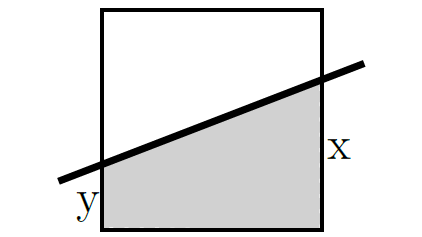
\includegraphics[scale = 0.5]{ProblemE.png}
	\par}
\end{figure*}

Answer:\\
Notice that $A(x,y)$ is a trapezoid.\\

The area of a trapezoid with lower base $p$, upper base $q$, and height $h$ is given by:

\begin{equation*}
	\frac{h}{2} \cdot (p + q)
\end{equation*}

Hence,
\begin{equation*}
	A(x,y) = \frac{a}{2} \cdot (x + y)
\end{equation*}

Alternatively, we can view the area $A(x,y)$ as the area of the square subtracted by the area of the white trapezoid, i.e.:

\begin{equation*}
	A(x,y) = a^2 - \frac{a}{2} \cdot ((a - x) + (a - y)) = a(a - \frac{2a - (x + y)}{2}) = a(\frac{x + y}{2} = \frac{a}{2}(x + y)
\end{equation*}

which yields the same result as it should.\\

$\therefore$ The surface area $A(x,y)$ below the line is given by the expression:

\begin{equation*}
	A(x,y) = \frac{a}{2}(x + y)
\end{equation*}


\end{document}